% !TeX spellcheck = cs_CZ
\begin{example}\label{AES:exam001}
  Proveďte simulaci vyznačených obvodových veličin obvodu na obrá\-zku \ref{AES:fig_exam001_1} se 
  zadanými hodnotami prvků v programu  PSpice\footnote{Simulace je provedena v programu 
  \texttt{OrCAD PSpice} ver. 16.3}.

   {\centering
    \captionsetup{type=figure} 
    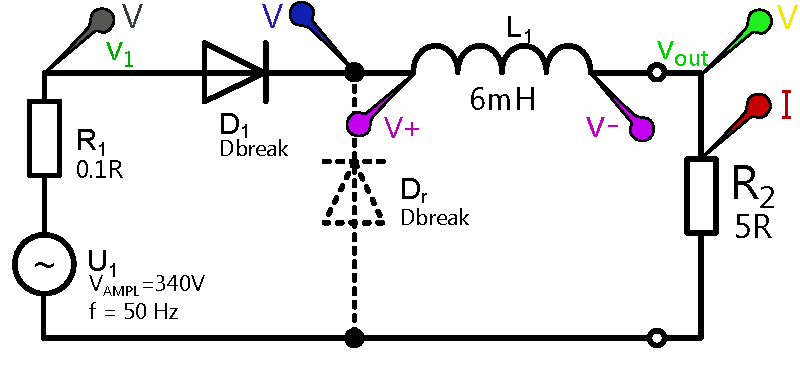
\includegraphics[width=0.8\linewidth]{patocka_jednocestny_1f_usm_PSpice.pdf}
    \captionof{figure}{Neřízený Jednofázový usměrňovač s nulovou diodu. Simulované veličiny jsou 
               vyznačeny barevnými markery.}
    \label{AES:fig_exam001_1}
    \par}

   {\centering
    \captionsetup{type=figure} 
    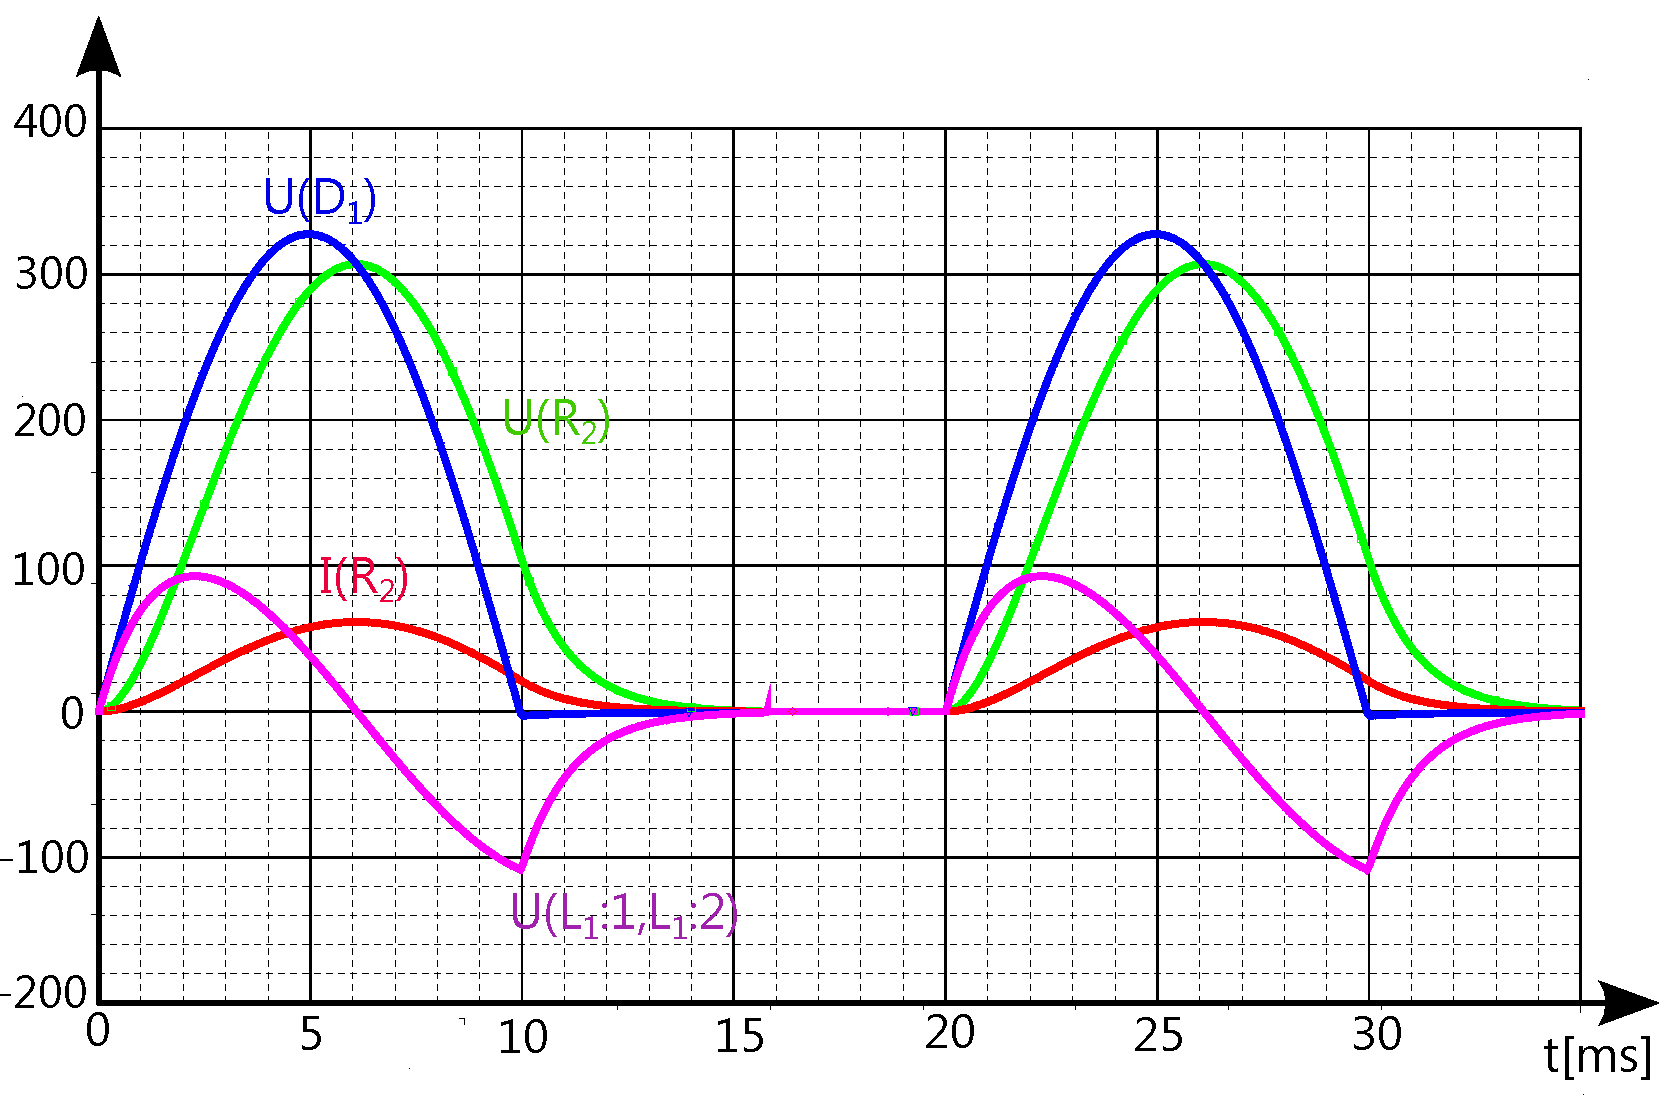
\includegraphics[width=0.9\linewidth]{PSPice_SIM002_usm1f_RL_6mH_5R.pdf}
    \captionof{figure}{Průběhy vyznačených veličin jednofázového neřízeného usměrňovače s RL zátěží 
              (6mH, 5$\Omega$) a nulovou diodou [ENZ/SIM002]}
    \label{AES:fig_exam001_2}
    \par}
\end{example}